\begin{frame}{Mein Aufgabenbereich}
	\begin{itemize}
		\item Implementierung des Agenten Horse und seiner Attribute
		\item Serialisierung/Deserialisierung Horse/AttributesHorse
	\end{itemize}

	\begin{tabular}{ccc}
		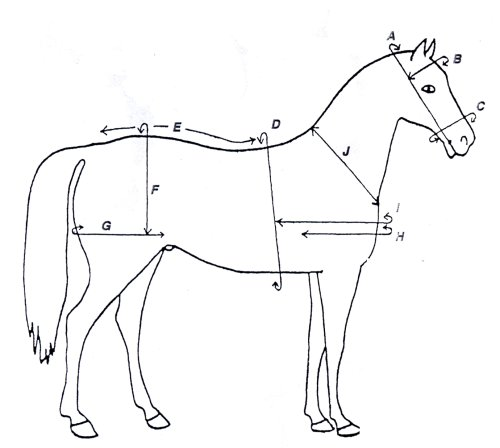
\includegraphics[width=125px, height=150px, keepaspectratio]{appendix/images/pferd.jpg}
		
\includegraphics[width=50px, height=50px, keepaspectratio]{appendix/images/pfeil-links-rechts.jpg}
		\hspace{0.7em}
		
\includegraphics[width=150px, height=75px, keepaspectratio]{appendix/images/horse-in-box.png}
	\end{tabular}

\end{frame}

\begin{frame}{Bisheriger Stand}
	\begin{itemize}
		\item Zwei dynamische Szenario Elemente "Pedestrian" und "Car"
		\item Ersteres für die Personenstromsimulation
		\item Letzeres für die Simulation des Kraftfahrzeugverkehrs (Peter Zarnitz) \cite{zarnitz-2015}
	\end{itemize}
\end{frame}

\begin{frame}{Anforderung}
	\begin{enumerate}
		\item Neuer Agent läuft im Backend (Simulator)
		\item Der Agent kann in die GUI aufgenommen werden
		\item Attribute des Agenten in der GUI editierbar
	\end{enumerate}
\end{frame}

\begin{frame}{Umsetzung: UML Szenario Elemente}
	\begin{figure}
		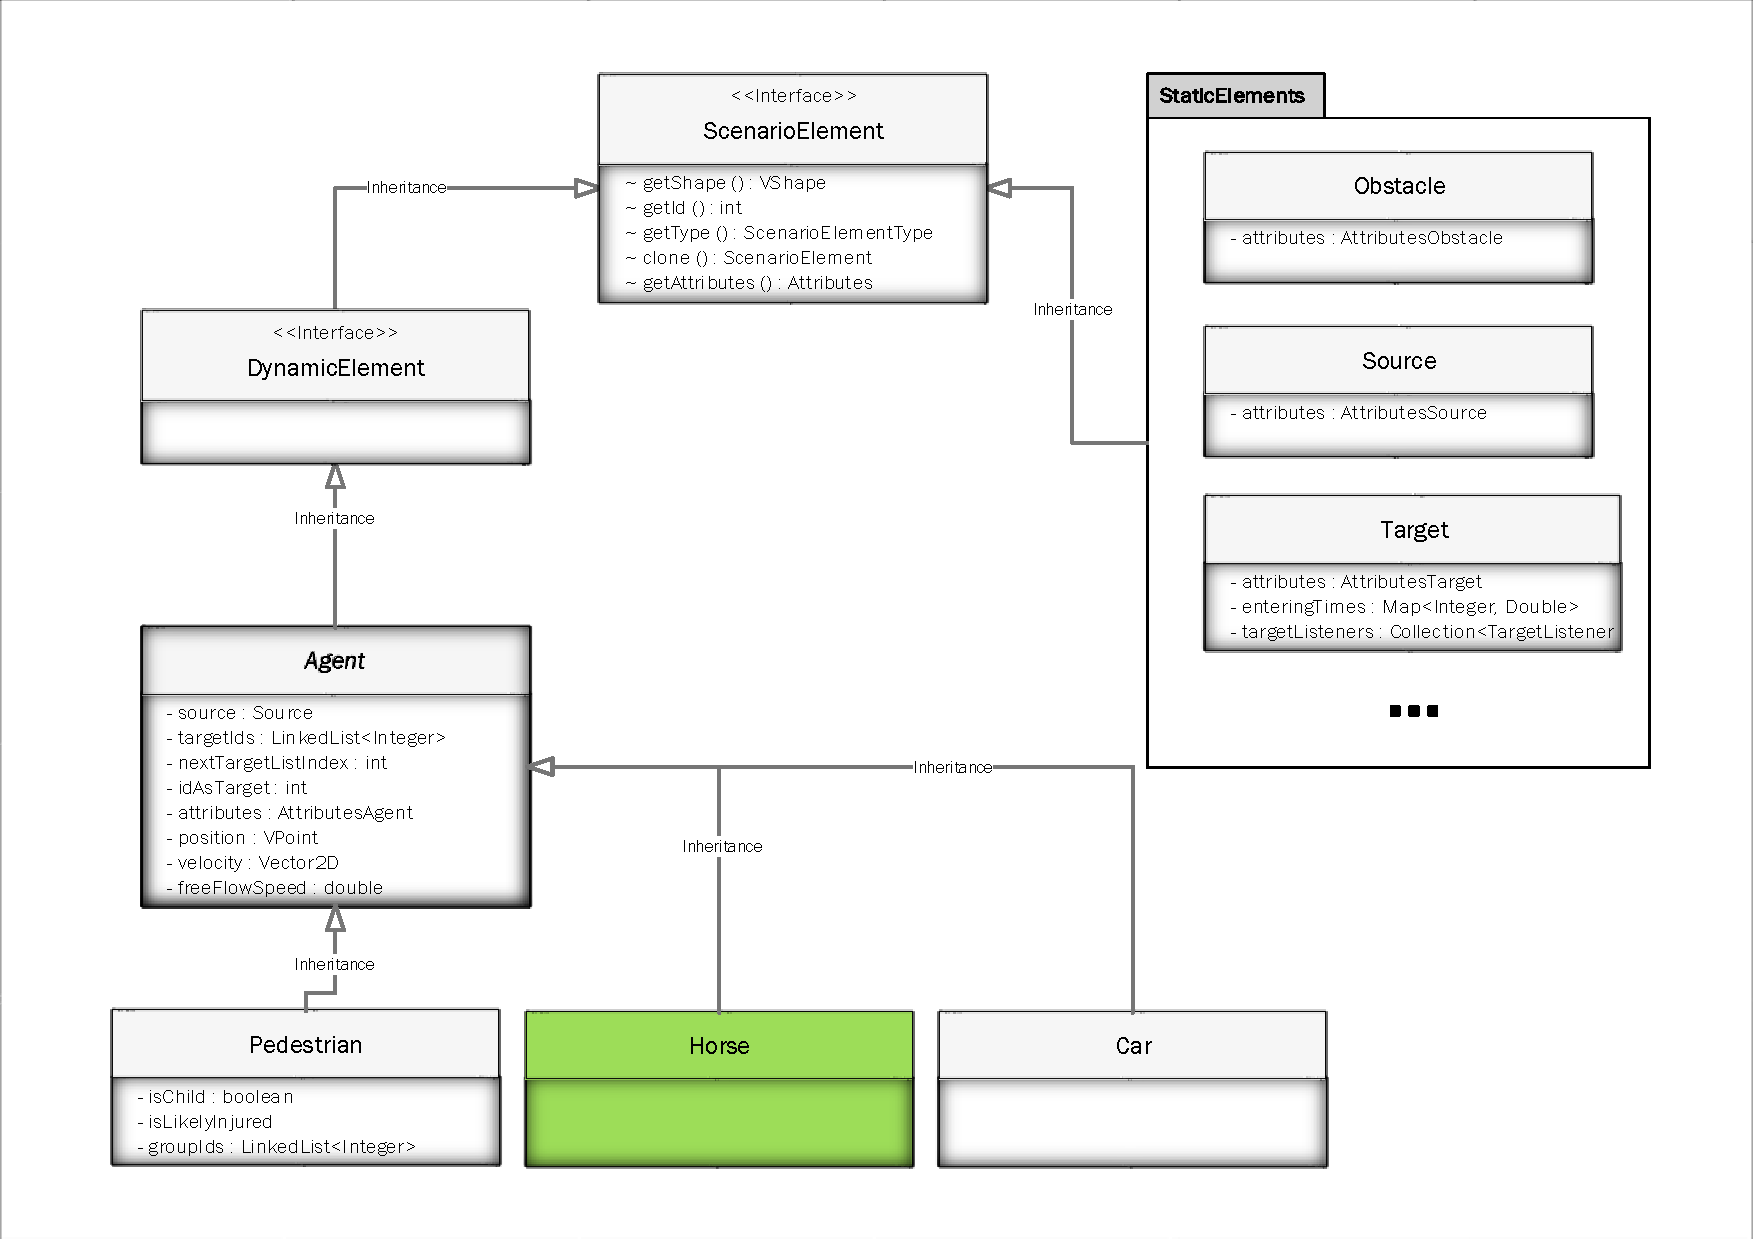
\includegraphics[width=\textwidth, keepaspectratio]{appendix/uml/ScenarioElements.pdf}
	\end{figure}
\end{frame}

\begin{frame}{Umsetzung: UML Attribute}
	\begin{figure}
		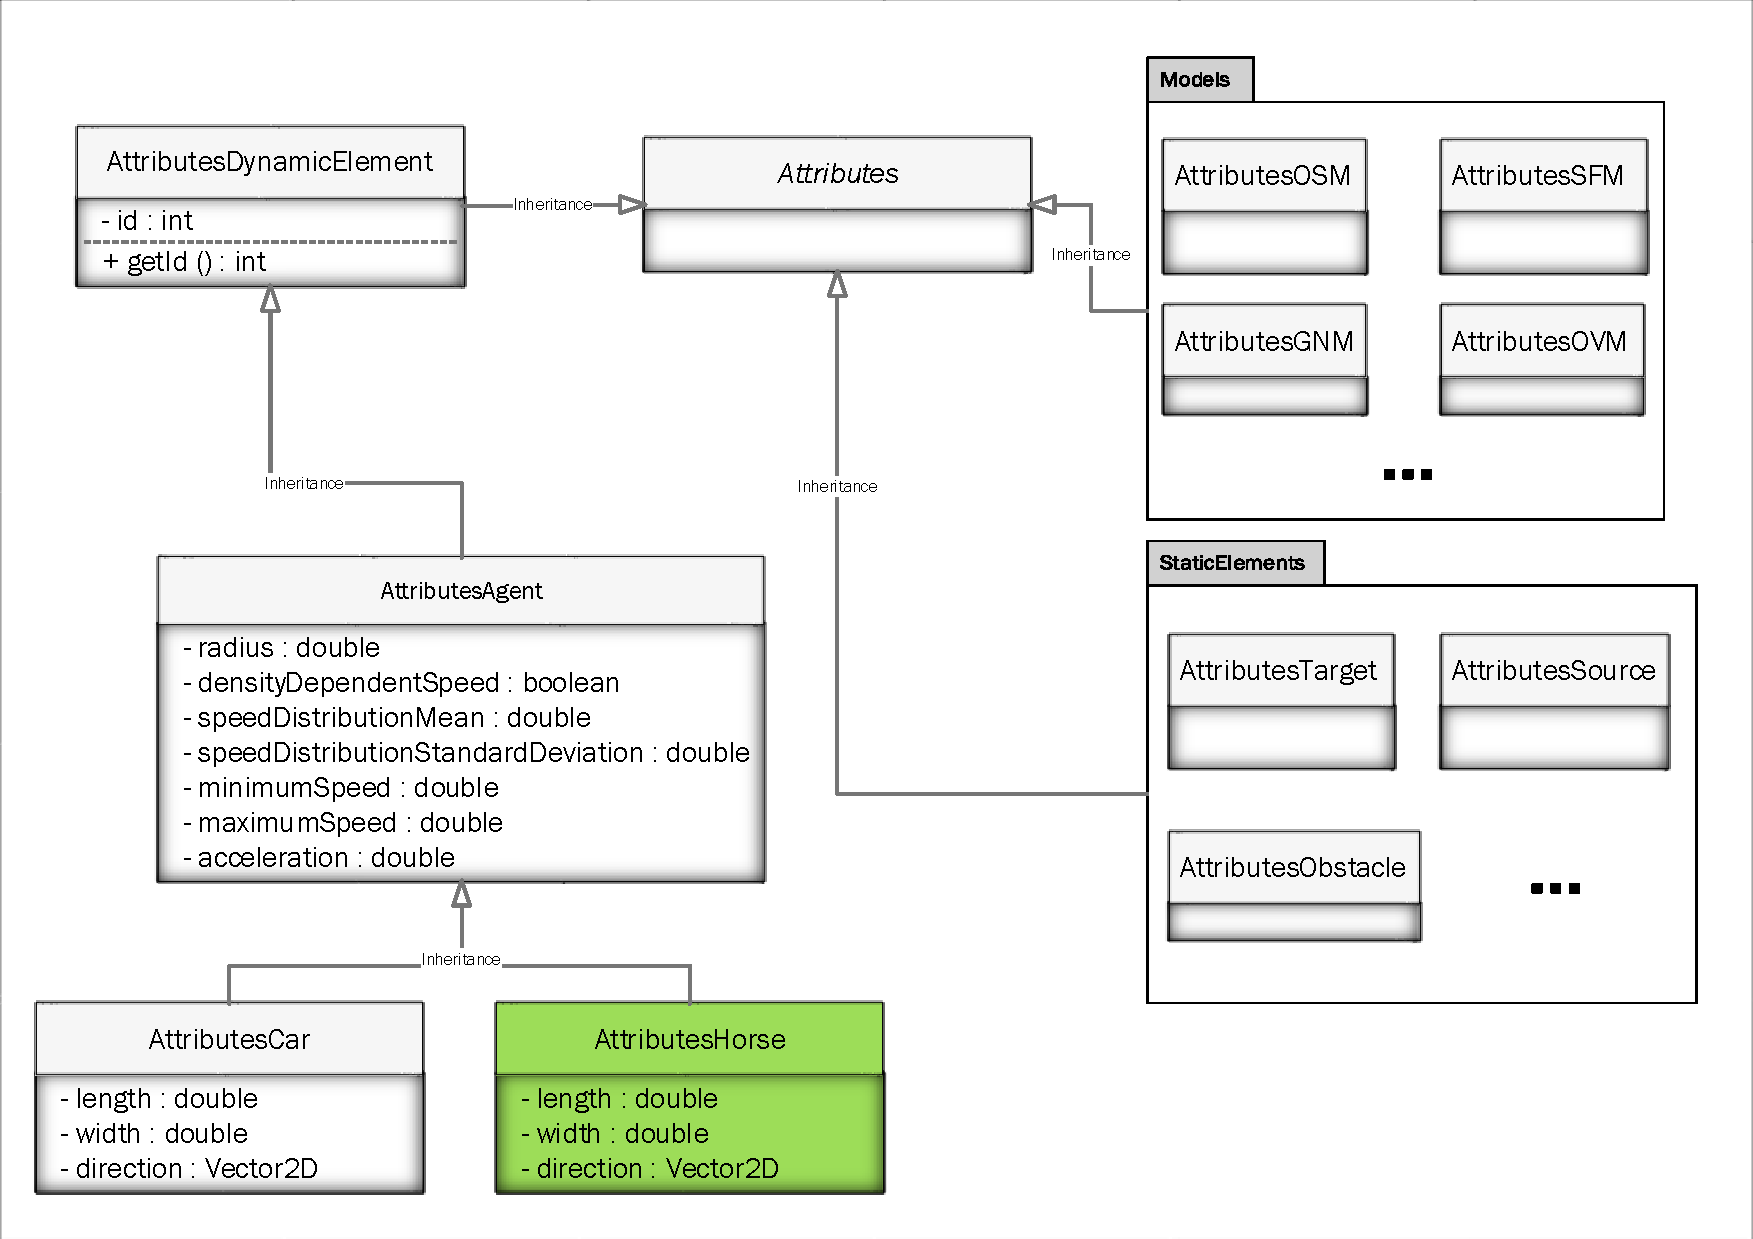
\includegraphics[width=\textwidth, keepaspectratio]{appendix/uml/Attributes.pdf}
	\end{figure}
\end{frame}

\begin{frame}{Ergebnisse}
	\begin{itemize}
		\item	Das Pferd kann in der Simulation, sowie in der GUI wie ein Fußgänger einbezogen werden
		\item Die Eigenschaften der Klassen Horse und AttributesHorse können serialisiert werden
		\item Das Pferd trägt zur Zeit die selben Eigenschaften wie ein Auto/Fußgänger
	\end{itemize}
\end{frame}

\begin{frame}{Fazit}
	\begin{itemize}
		\item Der Vorgang zum Einbetten eines neuen Agenten ist klar geworden
		\item Das derzeitige Fehlverhalten des Pferdes ist beabsichtigt
		\item Tatsächliche Maße und Eigenschaften des Pferdes können angepasst werden
	\end{itemize}
\end{frame}
